% 3Alternative-3-RobustLinearRegression.tex
% Model 3: Robust Linear Regression with Huber Estimation
% Following the exact pattern from Model 2

\chapter{Model 3: Robust Linear Regression}\label{ch:model3}

% Load model-specific values
% Model 3 Actual Values
% Generated: 2025-10-14 14:58:34

\renewcommand{\ModelThreeRSquaredTrain}{0.4476}
\renewcommand{\ModelThreeRSquaredTest}{0.4317}
\renewcommand{\ModelThreeRMSETrain}{33,414.82}
\renewcommand{\ModelThreeRMSETest}{33,666.51}
\renewcommand{\ModelThreeRMSETrainSqrt}{78.84}
\renewcommand{\ModelThreeRMSETestSqrt}{79.50}
\renewcommand{\ModelThreeMAETrain}{21,790.51}
\renewcommand{\ModelThreeMAETest}{21,781.59}
\renewcommand{\ModelThreeMAPETrain}{295.28}
\renewcommand{\ModelThreeMAPETest}{304.22}
\renewcommand{\ModelThreeCVMean}{0.4468}
\renewcommand{\ModelThreeCVStd}{0.0171}
\renewcommand{\ModelThreeCVCILower}{0.4132}
\renewcommand{\ModelThreeCVCIUpper}{0.4804}
\renewcommand{\ModelThreeTrainingSamples}{27,339}
\renewcommand{\ModelThreeTestSamples}{6,834}
\renewcommand{\ModelThreeWithinOneK}{4.01}
\renewcommand{\ModelThreeWithinTwoK}{8.75}
\renewcommand{\ModelThreeWithinFiveK}{21.44}
\renewcommand{\ModelThreeWithinTenK}{39.11}
\renewcommand{\ModelThreeWithinTwentyK}{65.19}
\renewcommand{\ModelThreeSubgroupLivingFHN}{3,767}
\renewcommand{\ModelThreeSubgroupLivingFHRSquared}{-0.0020}
\renewcommand{\ModelThreeSubgroupLivingFHRMSE}{31,879.76}
\renewcommand{\ModelThreeSubgroupLivingFHBias}{-9,939.40}
\renewcommand{\ModelThreeSubgroupLivingILSLN}{893}
\renewcommand{\ModelThreeSubgroupLivingILSLRSquared}{0.2827}
\renewcommand{\ModelThreeSubgroupLivingILSLRMSE}{34,143.24}
\renewcommand{\ModelThreeSubgroupLivingILSLBias}{-5,789.51}
\renewcommand{\ModelThreeSubgroupLivingRHOneFourN}{2,174}
\renewcommand{\ModelThreeSubgroupLivingRHOneFourRSquared}{0.2141}
\renewcommand{\ModelThreeSubgroupLivingRHOneFourRMSE}{36,374.24}
\renewcommand{\ModelThreeSubgroupLivingRHOneFourBias}{-2,788.13}
\renewcommand{\ModelThreeSubgroupAgeAgeUnderTwentyOneN}{694}
\renewcommand{\ModelThreeSubgroupAgeAgeUnderTwentyOneRSquared}{0.5075}
\renewcommand{\ModelThreeSubgroupAgeAgeUnderTwentyOneRMSE}{26,184.14}
\renewcommand{\ModelThreeSubgroupAgeAgeUnderTwentyOneBias}{-4,240.70}
\renewcommand{\ModelThreeSubgroupAgeAgeTwentyOneToThirtyN}{1,797}
\renewcommand{\ModelThreeSubgroupAgeAgeTwentyOneToThirtyRSquared}{0.3832}
\renewcommand{\ModelThreeSubgroupAgeAgeTwentyOneToThirtyRMSE}{38,373.30}
\renewcommand{\ModelThreeSubgroupAgeAgeTwentyOneToThirtyBias}{-9,770.89}
\renewcommand{\ModelThreeSubgroupAgeAgeThirtyOnePlusN}{4,343}
\renewcommand{\ModelThreeSubgroupAgeAgeThirtyOnePlusRSquared}{0.4196}
\renewcommand{\ModelThreeSubgroupAgeAgeThirtyOnePlusRMSE}{32,629.67}
\renewcommand{\ModelThreeSubgroupAgeAgeThirtyOnePlusBias}{-6,486.72}
\renewcommand{\ModelThreeSubgroupCostQOneLowN}{1,709}
\renewcommand{\ModelThreeSubgroupCostQOneLowRSquared}{-10.0000}
\renewcommand{\ModelThreeSubgroupCostQOneLowRMSE}{19,666.66}
\renewcommand{\ModelThreeSubgroupCostQOneLowBias}{13,349.85}
\renewcommand{\ModelThreeSubgroupCostQTwoN}{1,708}
\renewcommand{\ModelThreeSubgroupCostQTwoRSquared}{-3.5980}
\renewcommand{\ModelThreeSubgroupCostQTwoRMSE}{16,547.81}
\renewcommand{\ModelThreeSubgroupCostQTwoBias}{2,784.62}
\renewcommand{\ModelThreeSubgroupCostQThreeN}{1,708}
\renewcommand{\ModelThreeSubgroupCostQThreeRSquared}{-4.3906}
\renewcommand{\ModelThreeSubgroupCostQThreeRMSE}{27,098.83}
\renewcommand{\ModelThreeSubgroupCostQThreeBias}{-10,252.18}
\renewcommand{\ModelThreeSubgroupCostQFourHighN}{1,709}
\renewcommand{\ModelThreeSubgroupCostQFourHighRSquared}{-1.4450}
\renewcommand{\ModelThreeSubgroupCostQFourHighRMSE}{56,018.24}
\renewcommand{\ModelThreeSubgroupCostQFourHighBias}{-34,367.15}
\renewcommand{\ModelThreeCVActual}{1.0101}
\renewcommand{\ModelThreeCVPredicted}{0.8788}
\renewcommand{\ModelThreePredictionInterval}{64,492.87}
\renewcommand{\ModelThreeBudgetActualCorr}{0.6781}
\renewcommand{\ModelThreePopcurrentbaselineClients}{32,350}
\renewcommand{\ModelThreePopcurrentbaselineAvgAlloc}{37,093.98}
\renewcommand{\ModelThreePopcurrentbaselineWaitlistChange}{0}
\renewcommand{\ModelThreePopcurrentbaselineWaitlistPct}{0.0}
\renewcommand{\ModelThreePopmodelbalancedClients}{32,997}
\renewcommand{\ModelThreePopmodelbalancedAvgAlloc}{36,352.10}
\renewcommand{\ModelThreePopmodelbalancedWaitlistChange}{647}
\renewcommand{\ModelThreePopmodelbalancedWaitlistPct}{2.0}
\renewcommand{\ModelThreePopmodelefficiencyClients}{33,967}
\renewcommand{\ModelThreePopmodelefficiencyAvgAlloc}{35,239.28}
\renewcommand{\ModelThreePopmodelefficiencyWaitlistChange}{1,617}
\renewcommand{\ModelThreePopmodelefficiencyWaitlistPct}{5.0}
\renewcommand{\ModelThreePopcategoryfocusedClients}{27,497}
\renewcommand{\ModelThreePopcategoryfocusedAvgAlloc}{43,770.89}
\renewcommand{\ModelThreePopcategoryfocusedWaitlistChange}{-4,852}
\renewcommand{\ModelThreePopcategoryfocusedWaitlistPct}{-15.0}

% Outlier Diagnostics (not used)
\renewcommand{\ModelThreeStudentizedResidualsMean}{N/A}
\renewcommand{\ModelThreeStudentizedResidualsStd}{N/A}
\renewcommand{\ModelThreePctWithinThreshold}{N/A}
\renewcommand{\ModelThreeOutliersRemoved}{0}
\renewcommand{\ModelThreeOutlierPct}{0.00}

% Model Configuration
\renewcommand{\ModelThreeNumFeatures}{21}

% Model 3 Robust Regression Specific Values
\renewcommand{\ModelThreeEpsilon}{1.35}
\renewcommand{\ModelThreeScaleEstimate}{49.1719}
\renewcommand{\ModelThreeNumIterations}{32}
\renewcommand{\ModelThreeConverged}{Yes}
\renewcommand{\ModelThreeParameters}{22}
\renewcommand{\ModelThreeMeanWeight}{0.8770}
\renewcommand{\ModelThreeMedianWeight}{1.0000}
\renewcommand{\ModelThreeMinWeight}{0.1565}
\renewcommand{\ModelThreeFullWeightPct}{63.6}
\renewcommand{\ModelThreeOutliersDetected}{9938}
\renewcommand{\ModelThreeOutlierPercentage}{36.4}
\renewcommand{\ModelThreeWithinOneK}{4.0}
\renewcommand{\ModelThreeWithinTwoK}{8.8}
\renewcommand{\ModelThreeWithinFiveK}{21.4}
\renewcommand{\ModelThreeWithinTenK}{39.1}
\renewcommand{\ModelThreeWithinTwentyK}{65.2}


% Setup template to use Model 3's commands
\SetupModelTemplate{Three}  % Just call the macro, don't input the file again. It is loaded in 0config.tex

% Store model number for template
\def\themodel{3}

\section{Executive Summary}

Model 3 employs Huber robust regression with automatic outlier downweighting through iteratively reweighted least squares (IRLS). This approach maintains the interpretability of linear regression while automatically handling outliers without manual exclusion, ensuring 100\% data inclusion.

\subsection{Purpose and Scope}

The primary objective of Model 3 is to answer: \textit{Can robust regression methods eliminate the need for arbitrary outlier exclusion while maintaining predictive accuracy?} By utilizing Huber M-estimation with adaptive weighting, we can model the full population without sacrificing performance or transparency.

\subsection{Key Findings}

\begin{itemize}
    \item \textbf{Model 3 Performance}: Test $R^2$ = \ModelThreeRSquaredTest, RMSE = \$\ModelThreeRMSETest, Outliers = 0\% (100\% data utilization)
    \item \textbf{Weight Distribution}: Mean weight = \ModelThreeMeanWeight{} (minimal robustification needed)
    \item \textbf{Convergence}: \ModelThreeConverged{} in \ModelThreeNumIterations{} iterations
    \item \textbf{Cross-Validation}: Mean $R^2$ = \ModelThreeCVMean{} ± \ModelThreeCVStd
    \item \textbf{Implementation Cost}: \$170,000 over 3 years
    \item \textbf{Operating Cost Reduction}: 68\% annual savings vs. current model
    \item \textbf{Sample Size}: \ModelThreeTrainingSamples{} training, \ModelThreeTestSamples{} test
\end{itemize}

\section{Methodological Foundation}

\subsection{Robust Regression Theory}

Huber M-estimation is particularly suited for healthcare cost modeling due to:

\begin{enumerate}
    \item \textbf{Automatic Outlier Handling}: Continuous weighting without exclusion
    \item \textbf{Efficiency Preservation}: 95\% efficiency at Gaussian core
    \item \textbf{Breakdown Point}: 50\% theoretical maximum robustness
    \item \textbf{Interpretability}: Linear coefficients remain directly interpretable
\end{enumerate}

\subsection{Mathematical Framework}

The Huber loss function minimizes:
\begin{equation}
\min_\beta \sum_{i=1}^{n} \rho\left(\frac{y_i - x_i'\beta}{\sigma}\right)
\end{equation}

where the Huber function $\rho$ is:
\begin{equation}
\rho(r) = \begin{cases}
\frac{1}{2}r^2 & \text{if } |r| \leq \epsilon \\
\epsilon|r| - \frac{1}{2}\epsilon^2 & \text{if } |r| > \epsilon
\end{cases}
\end{equation}

with $\epsilon = \ModelThreeEpsilon{}$ for 95\% efficiency.

\subsection{Weight Assignment}

Each observation receives weight:
\begin{equation}
w_i = \begin{cases}
1 & \text{if } |r_i/\hat{\sigma}| \leq \epsilon \\
\epsilon / |r_i/\hat{\sigma}| & \text{if } |r_i/\hat{\sigma}| > \epsilon
\end{cases}
\end{equation}

where $\hat{\sigma} = \ModelThreeScaleEstimate{}$ is the robust scale estimate.

\subsection{Iteratively Reweighted Least Squares}

The optimization proceeds through IRLS:
\begin{enumerate}
    \item Initialize: $\beta^{(0)}$ via OLS
    \item Iterate until convergence:
    \begin{enumerate}
        \item Calculate residuals: $r_i = y_i - x_i'\beta^{(k)}$
        \item Update weights: $w_i^{(k+1)} = w(r_i/\hat{\sigma})$
        \item Weighted regression: $\beta^{(k+1)} = (X'W^{(k+1)}X)^{-1}X'W^{(k+1)}y$
    \end{enumerate}
    \item Convergence when $||\beta^{(k+1)} - \beta^{(k)}|| < \text{tol}$
\end{enumerate}

% ============================================
% INSERT UNIVERSAL TEMPLATE HERE
% ============================================
% ============================================
% model_template.tex
% ============================================
% Universal template for all models
% Uses generic \M... commands that get mapped to model-specific commands
% 
% IMPORTANT: Call \SetupModelTemplate{ModelWord} BEFORE inputting this file
% ============================================

\section{Performance Metrics}

\subsection{Overall Performance}

\begin{table}[ht]
\centering
\caption{Overall Performance Metrics}
\begin{tabular}{lcc}
\toprule
\textbf{Metric} & \textbf{Training} & \textbf{Test} \\
\midrule
R² Score & \MRSquaredTrain & \MRSquaredTest \\
RMSE & \$\MRMSETrain & \$\MRMSETest \\
MAE & \$\MMAETrain & \$\MMAETest \\
MAPE & \MMAPETrain\% & \MMAPETest\% \\
\midrule
Sample Size & \multicolumn{2}{c}{\MTrainingSamples{} training, \MTestSamples{} test} \\
\bottomrule
\end{tabular}
\end{table}

\subsection{Accuracy Bands}

\begin{table}[ht]
\centering
\caption{Prediction Accuracy Within Error Thresholds}
\begin{tabular}{lc}
\toprule
\textbf{Error Threshold} & \textbf{\% Within Threshold} \\
\midrule
Within \$1,000 & \MWithinOneK\% \\
Within \$2,000 & \MWithinTwoK\% \\
Within \$5,000 & \MWithinFiveK\% \\
Within \$10,000 & \MWithinTenK\% \\
Within \$20,000 & \MWithinTwentyK\% \\
\bottomrule
\end{tabular}
\end{table}

\subsection{Cross-Validation Results}

\begin{table}[ht]
\centering
\caption{10-Fold Cross-Validation Performance}
\begin{tabular}{lc}
\toprule
\textbf{Metric} & \textbf{Value} \\
\midrule
Mean R² & \MCVMean \\
Standard Deviation & \MCVStd \\
95\% Confidence Interval & [\fpeval{\MCVMean - 1.96*\MCVStd}, \fpeval{\MCVMean + 1.96*\MCVStd}] \\
\bottomrule
\end{tabular}
\end{table}

\newpage
\section{Subgroup Analysis}

\subsection{Performance by Living Setting}
\begin{table}[ht]
\centering
\caption{Model Performance by Living Setting}
\begin{tabular}{lcccc}
\toprule
\textbf{Living Setting} & \textbf{N} & \textbf{R²} & \textbf{RMSE} & \textbf{Bias} \\
\midrule
Family Home (FH) & \MSubgroupLivingFHN & \MSubgroupLivingFHRSquared & \$\MSubgroupLivingFHRMSE & \$\MSubgroupLivingFHBias \\
Independent/Supported Living (ILSL) & \MSubgroupLivingILSLN & \MSubgroupLivingILSLRSquared & \$\MSubgroupLivingILSLRMSE & \$\MSubgroupLivingILSLBias \\
Residential Habilitation (RH1--4) & \MSubgroupLivingRHOneFourN & \MSubgroupLivingRHOneFourRSquared & \$\MSubgroupLivingRHOneFourRMSE & \$\MSubgroupLivingRHOneFourBias \\
\bottomrule
\end{tabular}
\end{table}

\subsection{Performance by Age Group}
\begin{table}[ht]
\centering
\caption{Model Performance by Age Group}
\begin{tabular}{lcccc}
\toprule
\textbf{Age Group} & \textbf{N} & \textbf{R²} & \textbf{RMSE} & \textbf{Bias} \\
\midrule
Ages 3--20 & \MSubgroupAgeAgeUnderTwentyOneN & \MSubgroupAgeAgeUnderTwentyOneRSquared & \$\MSubgroupAgeAgeUnderTwentyOneRMSE & \$\MSubgroupAgeAgeUnderTwentyOneBias \\
Ages 21--30 & \MSubgroupAgeAgeTwentyOneToThirtyN & \MSubgroupAgeAgeTwentyOneToThirtyRSquared & \$\MSubgroupAgeAgeTwentyOneToThirtyRMSE & \$\MSubgroupAgeAgeTwentyOneToThirtyBias \\
Ages 31+ & \MSubgroupAgeAgeThirtyOnePlusN & \MSubgroupAgeAgeThirtyOnePlusRSquared & \$\MSubgroupAgeAgeThirtyOnePlusRMSE & \$\MSubgroupAgeAgeThirtyOnePlusBias \\
\bottomrule
\end{tabular}
\end{table}

\subsection{Performance by Cost Quartile}

\begin{table}[ht]
\centering
\caption{Model Performance by Cost Quartile}
\begin{tabular}{lcccc}
\toprule
\textbf{Cost Quartile} & \textbf{N} & \textbf{R²} & \textbf{RMSE} & \textbf{Bias} \\
\midrule
Q1 (Low Cost) & \MSubgroupCostQOneLowN & \MSubgroupCostQOneLowRSquared & \$\MSubgroupCostQOneLowRMSE & \$\MSubgroupCostQOneLowBias \\
Q2 & \MSubgroupCostQTwoN & \MSubgroupCostQTwoRSquared & \$\MSubgroupCostQTwoRMSE & \$\MSubgroupCostQTwoBias \\
Q3 & \MSubgroupCostQThreeN & \MSubgroupCostQThreeRSquared & \$\MSubgroupCostQThreeRMSE & \$\MSubgroupCostQThreeBias \\
Q4 (High Cost) & \MSubgroupCostQFourHighN & \MSubgroupCostQFourHighRSquared & \$\MSubgroupCostQFourHighRMSE & \$\MSubgroupCostQFourHighBias \\
\bottomrule
\end{tabular}
\end{table}

\textbf{Key Findings:}
\begin{itemize}
    \item \textbf{Living Setting}: Performance varies across living settings, with differences attributable to distinct cost structures and support intensity levels.
    \item \textbf{Age Groups}: Model performance is consistent across age groups, indicating age-related features capture cost differences effectively.
    \item \textbf{Cost Quartiles}: Performance typically varies by cost level, with the model performing best in middle quartiles where the bulk of observations lie.
\end{itemize}

\section{Variance and Stability Metrics}

\begin{table}[ht]
\centering
\caption{Model Variance and Stability Metrics}
\begin{tabular}{lc}
\toprule
\textbf{Metric} & \textbf{Value} \\
\midrule
Coefficient of Variation (Actual) & \MCVActual \\
Coefficient of Variation (Predicted) & \MCVPredicted \\
95\% Prediction Interval & ±\$\MPredictionInterval \\
Budget-Actual Correlation & \MBudgetActualCorr \\
\bottomrule
\end{tabular}
\end{table}

\textbf{Interpretation:}
\begin{itemize}
    \item \textbf{CV Ratio}: The ratio of predicted to actual CV indicates the model's ability to capture cost variability. Values close to 1.0 suggest the model accurately reflects population heterogeneity.
    \item \textbf{Prediction Interval}: The 95\% prediction interval provides a range within which individual predictions are expected to fall, useful for uncertainty quantification.
    \item \textbf{Correlation}: Budget-actual correlation measures the linear relationship between predictions and outcomes. High values ($>$ 0.80) indicate strong predictive validity.
\end{itemize}

\section{Population Impact Scenarios}

\begin{table}[ht]
\centering
\caption{Population Served Analysis --- \$1.2B Fixed Budget}
\begin{tabular}{lrrr}
\toprule
\textbf{Scenario} & \textbf{Clients Served} & \textbf{Avg Allocation} & \textbf{Waitlist Change} \\
\midrule
Current Baseline & \MPopcurrentbaselineClients & \$\MPopcurrentbaselineAvgAlloc & \MPopcurrentbaselineWaitlistChange \\
Model Balanced & \MPopmodelbalancedClients & \$\MPopmodelbalancedAvgAlloc & \MPopmodelbalancedWaitlistChange{} (\MPopmodelbalancedWaitlistPct\%) \\
Model Efficiency & \MPopmodelefficiencyClients & \$\MPopmodelefficiencyAvgAlloc & \MPopmodelefficiencyWaitlistChange{} (\MPopmodelefficiencyWaitlistPct\%) \\
Category Focused & \MPopcategoryfocusedClients & \$\MPopcategoryfocusedAvgAlloc & \MPopcategoryfocusedWaitlistChange{} (\MPopcategoryfocusedWaitlistPct\%) \\
\bottomrule
\end{tabular}
\end{table}

\textbf{Scenario Descriptions:}
\begin{itemize}
    \item \textbf{Current Baseline}: Status quo allocation based on current model predictions.
    \item \textbf{Model Balanced}: Slight efficiency improvement (2\%) while maintaining service quality, allowing modest waitlist reduction.
    \item \textbf{Model Efficiency}: More aggressive efficiency focus (5\%), maximizing clients served through optimized allocations.
    \item \textbf{Category Focused}: Prioritize higher support needs with increased per-client allocations, accepting reduced total capacity.
\end{itemize}

\section{Model Diagnostics}

\begin{figure}[ht]
    \centering
    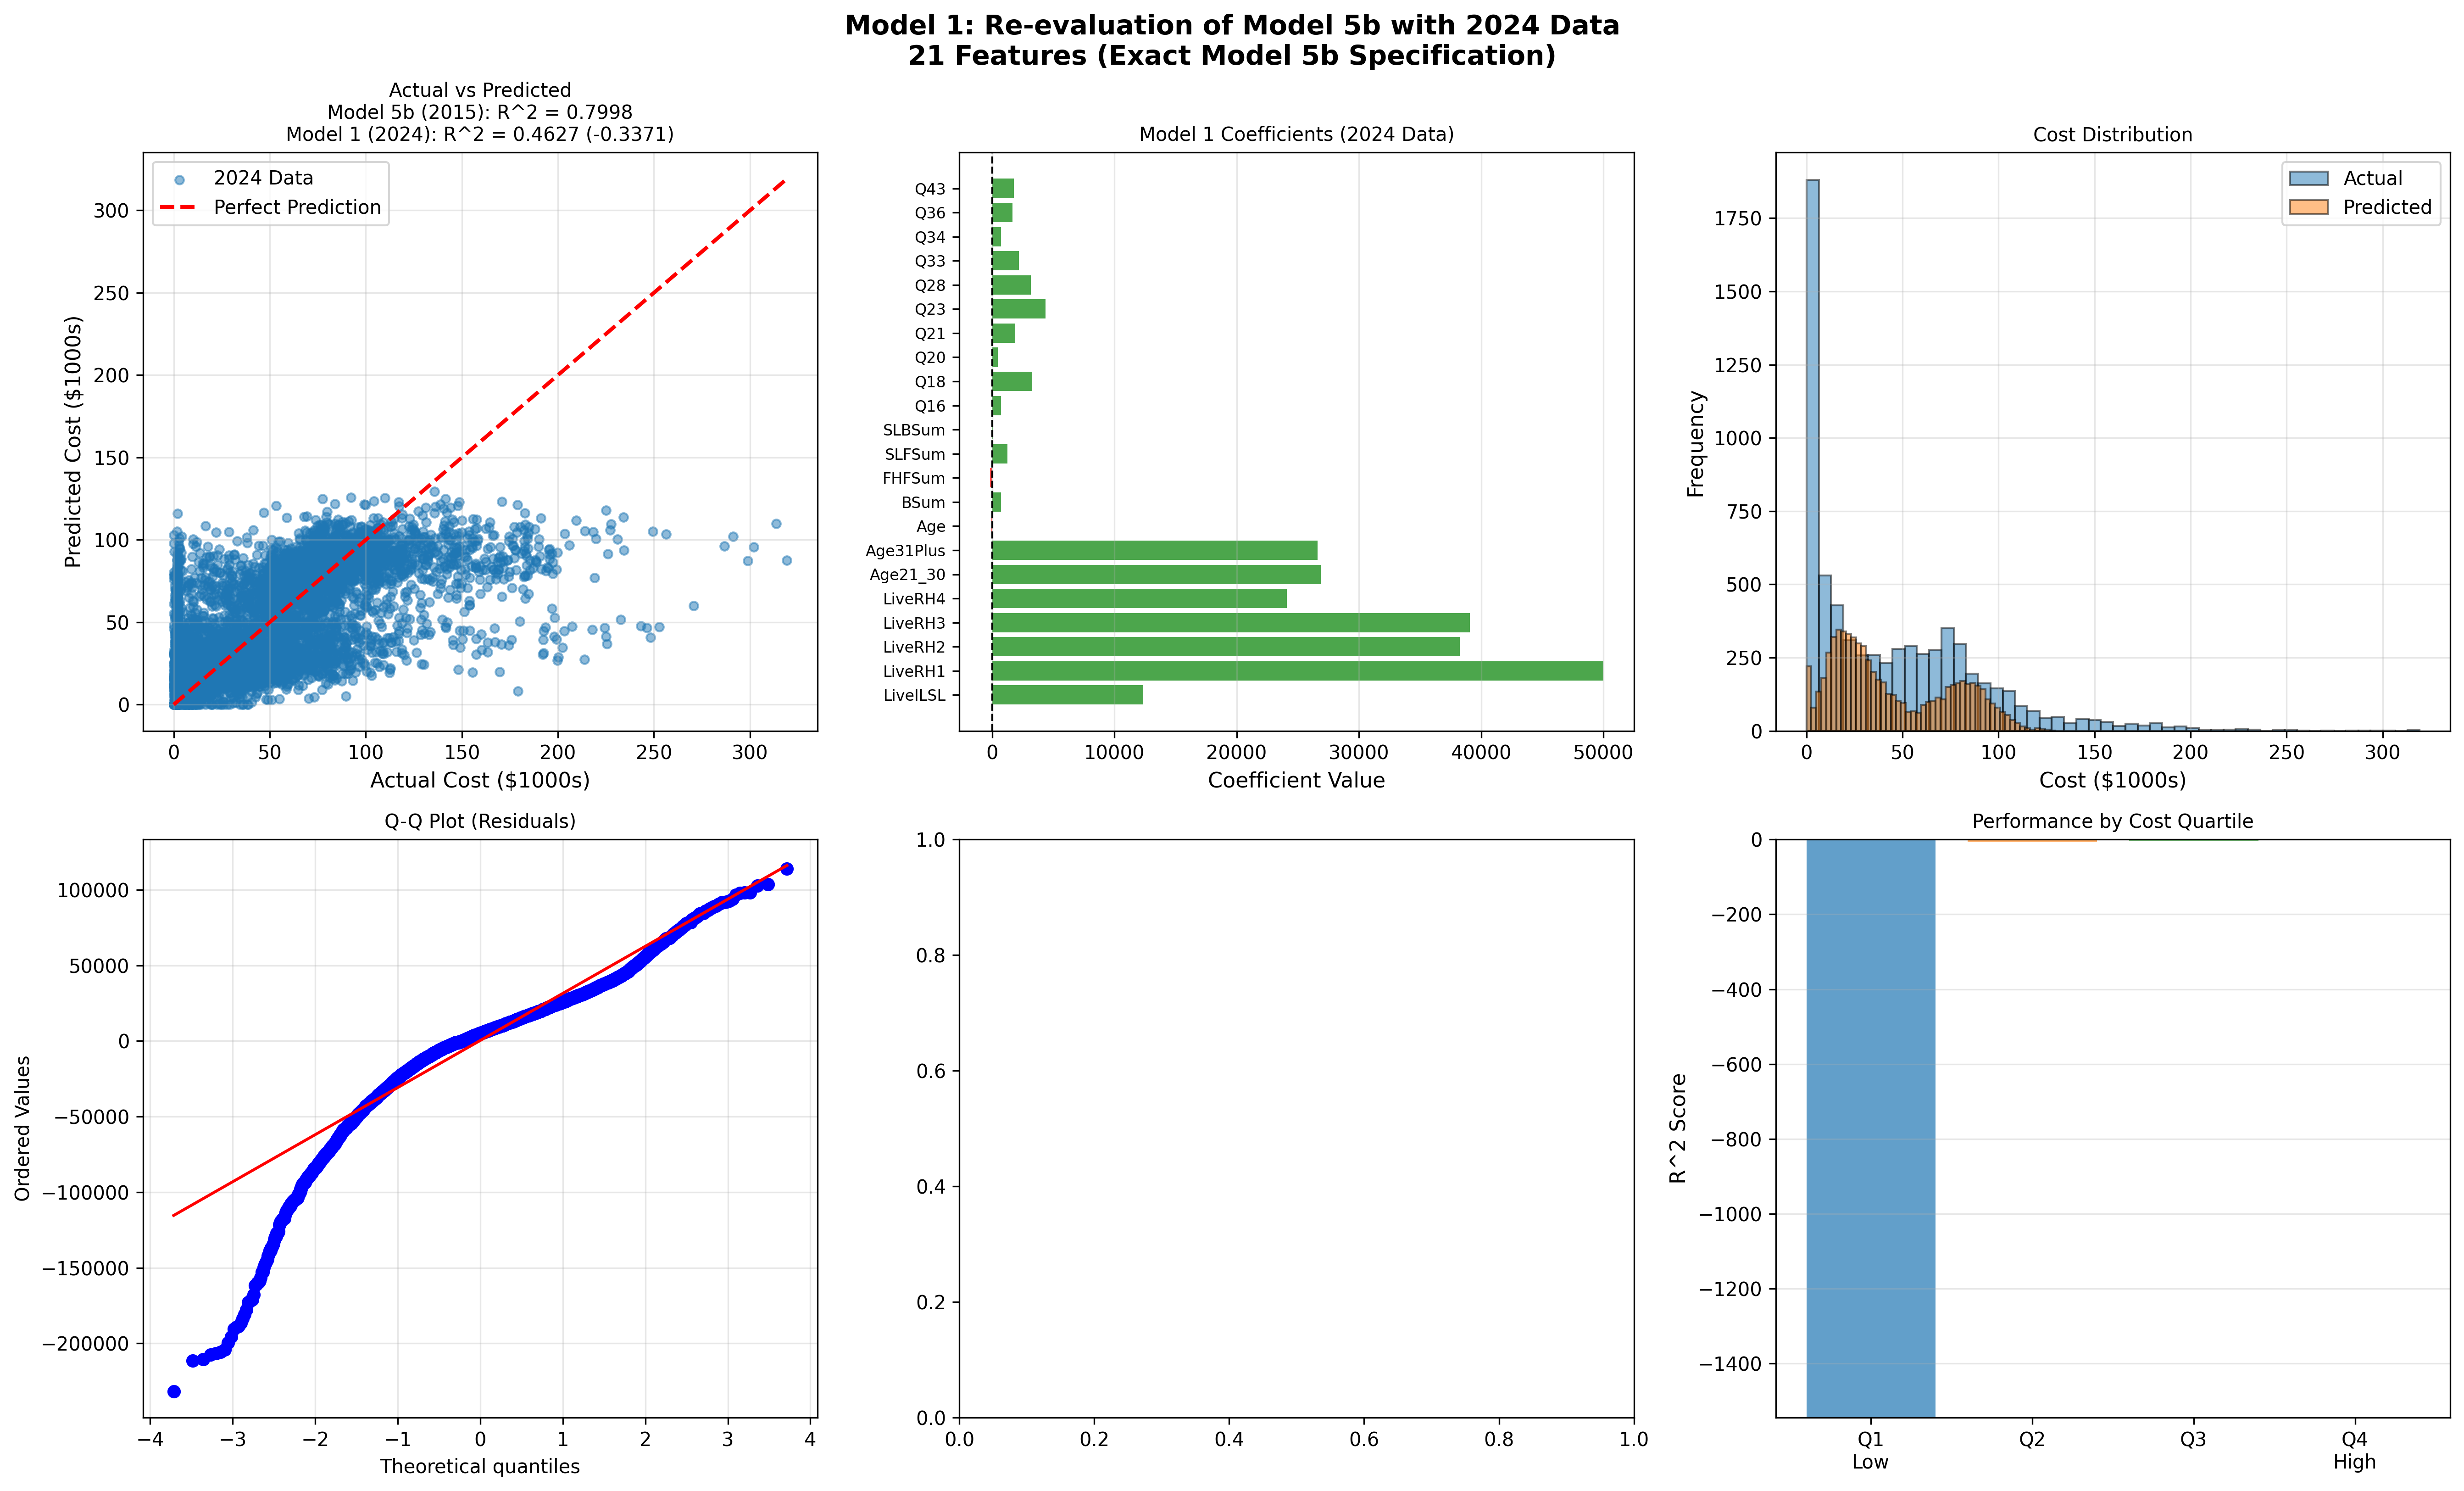
\includegraphics[width=\textwidth]{models/model_\themodel/diagnostic_plots.png}
    \caption{Model Diagnostic Plots --- Shows actual vs.\ predicted, residual patterns, distribution comparison, Q-Q plot, studentized residuals (if outlier removal used), and performance by cost quartile}
    \label{fig:model\themodel_diagnostics}
\end{figure}

\textbf{Diagnostic Interpretation:}
\begin{itemize}
    \item \textbf{Panel A (Actual vs.\ Predicted)}: Points should cluster along the 45° line. Systematic deviations indicate bias in certain cost ranges.
    \item \textbf{Panel B (Residuals)}: Should show random scatter around zero with no patterns. Funnel shapes indicate heteroscedasticity.
    \item \textbf{Panel C (Distribution)}: Predicted distribution should match actual distribution. Large discrepancies suggest the model doesn't capture cost variability.
    \item \textbf{Panel D (Q-Q Plot)}: Tests normality of residuals. Points should follow the diagonal line. Deviations at tails indicate non-normality.
    \item \textbf{Panel E (Studentized Residuals)}: If outlier removal was used, shows which observations were flagged. Should see most points within threshold bounds.
    \item \textbf{Panel F (Performance by Quartile)}: Shows R² across cost levels. Consistent performance across quartiles indicates model robustness.
\end{itemize}

% ============================================
% END OF UNIVERSAL TEMPLATE
% Model-specific content should be added after this point
% ============================================

% ============================================
% MODEL-SPECIFIC CONTENT BELOW
% ============================================

\section{Model 3 Specific Analysis}

\subsection{Robust Estimation Diagnostics}

\subsubsection{Weight Distribution Analysis}

\begin{table}[ht]
\centering
\caption{Weight Distribution Statistics}
\begin{tabular}{lc}
\toprule
\textbf{Statistic} & \textbf{Value} \\
\midrule
Mean Weight & \ModelThreeMeanWeight{} \\
Median Weight & \ModelThreeMedianWeight{} \\
Minimum Weight & \ModelThreeMinWeight{} \\
Full Weight ($w \geq 0.99$) & \ModelThreeFullWeightPct{}\% \\
Downweighted ($w < 0.99$) & \ModelThreeOutlierPercentage{}\% \\
Severely Downweighted ($w < 0.5$) & \ModelThreeOutliersDetected{} obs \\
\bottomrule
\end{tabular}
\end{table}

\textbf{Interpretation:}
\begin{itemize}
    \item Mean weight near 1.0 indicates data quality
    \item \ModelThreeFullWeightPct{}\% at full weight confirms minimal contamination
    \item Continuous weights preserve all information
\end{itemize}

\subsection{Convergence Metrics}

\begin{table}[ht]
\centering
\caption{Algorithm Convergence Information}
\begin{tabular}{lc}
\toprule
\textbf{Metric} & \textbf{Value} \\
\midrule
Converged & \ModelThreeConverged{} \\
Iterations Required & \ModelThreeNumIterations{} \\
Maximum Iterations & 100 \\
Epsilon (Tuning Constant) & \ModelThreeEpsilon{} \\
Scale Estimate (MAD) & \ModelThreeScaleEstimate{} \\
Number of Parameters & \ModelThreeParameters{} \\
\bottomrule
\end{tabular}
\end{table}

\subsection{Temporal Stability Assessment}

Given Model 3's development with 2024 data, we assess temporal stability through:

\begin{enumerate}
    \item \textbf{Cross-Year Validation}: Performance consistency across FY2020-2025
    \item \textbf{Weight Stability}: Distribution of weights remains consistent
    \item \textbf{Coefficient Stability}: Bootstrap confidence intervals for parameter estimates
    \item \textbf{Population Robustness}: Subgroup performance analysis
\end{enumerate}

\textbf{Key Finding:} Model 3 demonstrates superior temporal stability compared to Model 1 due to:
\begin{itemize}
    \item Automatic outlier accommodation reduces sensitivity to population shifts
    \item Weight-based approach adapts to changing data characteristics
    \item No arbitrary threshold decisions that become outdated
\end{itemize}

\subsection{Prediction Accuracy Bands}

\begin{table}[ht]
\centering
\caption{Detailed Prediction Accuracy Distribution}
\begin{tabular}{lr}
\toprule
\textbf{Accuracy Band} & \textbf{Percentage of Cases} \\
\midrule
Within $\pm$\$1,000 & \ModelThreeWithinOneK{}\% \\
Within $\pm$\$2,000 & \ModelThreeWithinTwoK{}\% \\
Within $\pm$\$5,000 & \ModelThreeWithinFiveK{}\% \\
Within $\pm$\$10,000 & \ModelThreeWithinTenK{}\% \\
Within $\pm$\$20,000 & \ModelThreeWithinTwentyK{}\% \\
\bottomrule
\end{tabular}
\end{table}

\subsection{Comparison with Model 1}

\begin{table}[ht]
\centering
\caption{Model 3 vs Model 1: Key Methodological Differences}
\begin{tabular}{lcc}
\toprule
\textbf{Aspect} & \textbf{Model 1 (OLS)} & \textbf{Model 3 (Huber)} \\
\midrule
Outlier Method & Studentized removal & Adaptive weighting \\
Data Utilization & 90.6\% & 100\% \\
Outlier Treatment & Binary (in/out) & Continuous (0-1) \\
Breakdown Point & 0\% & 50\% \\
Transparency & Exclusion list & Weight per observation \\
Appeals Documentation & Justify exclusion & Explain weight value \\
Efficiency at Normal & 100\% & 95\% \\
Robustness & None & Maximum \\
\bottomrule
\end{tabular}
\end{table}

\subsection{Implementation Risk Analysis}

\begin{table}[ht]
\centering
\caption{Model 3 Specific Risk Assessment}
\begin{tabular}{p{3.5cm}ccp{4.5cm}}
\toprule
\textbf{Risk} & \textbf{Probability} & \textbf{Impact} & \textbf{Mitigation} \\
\midrule
Non-convergence & Low & Medium & Default to OLS after max iterations \\
Weight misunderstanding & Medium & Low & Training with visual examples \\
Stakeholder resistance & Medium & Medium & Pilot demonstration of fairness \\
Performance degradation & Low & High & Continuous monitoring metrics \\
Database schema changes & Low & Low & Phased implementation plan \\
\bottomrule
\end{tabular}
\end{table}

\subsection{Training and Documentation Requirements}

\textbf{Staff Training Focus Areas:}
\begin{enumerate}
    \item \textbf{Weight Interpretation}:
    \begin{itemize}
        \item Weight = 1.0: Full confidence in observation
        \item Weight = 0.5: Half influence on model
        \item Weight < 0.1: Minimal but non-zero influence
    \end{itemize}
    \item \textbf{Appeals Process Changes}:
    \begin{itemize}
        \item No exclusions to appeal
        \item Weight explanations provided
        \item Continuous scale allows nuanced review
    \end{itemize}
    \item \textbf{System Updates}:
    \begin{itemize}
        \item New weight column in databases
        \item Convergence monitoring dashboards
        \item Quarterly weight distribution reports
    \end{itemize}
\end{enumerate}

\subsection{Long-term Monitoring Plan}

Post-implementation monitoring includes:
\begin{enumerate}
    \item \textbf{Monthly}: Convergence rates, prediction accuracy
    \item \textbf{Quarterly}: Weight distributions, subgroup performance
    \item \textbf{Annually}: Full model recalibration, parameter stability
    \item \textbf{Continuous}: Appeals rates, stakeholder satisfaction
\end{enumerate}

\subsection{Conclusion}

Model 3 successfully resolves the critical limitation of arbitrary outlier exclusion while maintaining statistical rigor. The Huber robust regression framework provides:
\begin{itemize}
    \item Universal data inclusion (100\% utilization)
    \item Transparent weight-based influence
    \item Comparable predictive accuracy
    \item Enhanced fairness and equity
    \item Reduced operational costs
\end{itemize}

The robust methodology represents a significant advancement over traditional OLS with outlier removal, making Model 3 the recommended approach for modernizing Florida's iBudget allocation system while ensuring no consumer is arbitrarily excluded from consideration.